\section{Evaluation}
\label{sec:eval}

We evaluate with two instruments. The \emph{agent study}
(\S\ref{sec:eval:setup}--\S\ref{sec:eval:revisions}) drives every protocol
with real language-model agents and answers four questions:
\begin{description}
\item[RQ1] Does certified chopping prevent the anomalies that uncoordinated
  agents produce, and how does it compare with locking and with repair?
\item[RQ2] What does it cost in time and tokens?
\item[RQ3] How do the three locking disciplines of
  \S\ref{sec:runtime:locking} differ?
\item[RQ4] How much does each protocol's correctness depend on the model?
\end{description}
The \emph{mechanism study} (\S\ref{sec:eval:mechanism}) uses the durable
runtime with real threads and a calibrated reasoning delay to measure
throughput at higher concurrency, admission rates under controlled
contention, certification cost and crash recovery.

\subsection{Agent study: setup}
\label{sec:eval:setup}

\paragraph{Workloads.}
Each workload, which we call a \emph{cell}, gives two agents natural-language
tasks over a small shared state and a set of tools. Table~\ref{tab:cells}
lists the twelve cells. Ten are \emph{contended}: they follow the methodology
of CoAgent's contended cells~\cite{lyu2026coagent}, with operations drawn from
cloud operations in the style of AIOpsLab~\cite{chen2025aiopslab} and
workplace tasks in the style of WorkBench~\cite{styles2024workbench}, and
each is built so that an unlucky interleaving produces a specific anomaly.
Two are structural cells for chopping: \cell{cc-claim} has a short shared
dependency followed by private work, the shape of
Figure~\ref{fig:sc}(a), and \cell{cc-escalate} is the impossibility witness of
Figure~\ref{fig:witness} made executable.

\begin{table}[t]
\caption{The twelve cells. Each runs two concurrent agents.}
\label{tab:cells}
\small
\begin{tabular}{@{}lp{5.1cm}@{}}
\toprule
Cell & Anomaly an unlucky interleaving produces \\
\midrule
\cell{k8s-canary}            & stale read + missed range scan \\
\cell{k8s-port-misconfig}    & phantom insert + stale read \\
\cell{k8s-permission-revoke} & phantom insert + stale read \\
\cell{k8s-replica-scale}     & lost update \\
\cell{k8s-rollback-audit}    & non-idempotent append on a stale premise \\
\cell{wb-crm-dedupe}         & phantom insert + stale read \\
\cell{wb-calendar-doublebook}& lost update (double booking) \\
\cell{wb-email-triage}       & non-idempotent append on a stale premise \\
\cell{wb-analytics-restate}  & phantom insert + stale read \\
\cell{wb-project-rebalance}  & lost update \\
\midrule
\cell{cc-claim}              & none: short shared read, private work \\
\cell{cc-escalate}           & mid-flight escalation into a peer's committed footprint \\
\bottomrule
\end{tabular}
\end{table}

\paragraph{Protocols.}
All eight protocols run on the same middleware, tools and agents:
\textbf{Serial} (one agent at a time, the correctness and speed reference);
\textbf{Naive} (no coordination); \textbf{2PL} and \textbf{OCC}
(whole-workflow isolation with saga undo); \textbf{\mtpo}, our
re-implementation of CoAgent's protocol from its paper, since its code is not
public; and \cc, \cctwo and \ccs.

\paragraph{Agents and models.}
Agents are driven by Claude Haiku~4.5 with extended thinking, and by Claude
Sonnet~5 at low reasoning effort. The Haiku run covers all eight protocols;
the Sonnet run covers the six that existed when it was made, that is, all but
\cctwo and \ccs. Every (cell, protocol) pair is run for ten seeds: 962 trials
with Haiku and 720 with Sonnet, at a total API cost of \$24.89.

\paragraph{Time.}
The agent runtime is a discrete-event scheduler. The duration of each tool
call is the measured wall-clock latency of the model inference that produced
it, and an agent that is blocked waits on the same clock. The time of a trial
is its makespan on this clock. \emph{Speedup} for a cell is the median serial
time divided by the median protocol time; we use medians because a single
trial with a stuck agent moves a mean by orders of magnitude. Aggregate
speedup is the mean over cells.

\paragraph{Scoring.}
For each cell we compute the set of final states that the two serial orders
can produce. A trial is \emph{anomaly-free} if the part of its final state
that concurrency can corrupt matches one of them; for \cell{cc-escalate}, a
refused escalation that leaves the shared state untouched is anomaly-free,
because refusing is the mechanism working. This predicate deliberately ignores
errors an agent makes on its own, which we measure separately as assumption A1
(\S\ref{sec:eval:agent}).

The predicate is trustworthy only if serial execution always satisfies it.
With Haiku, serial execution fails it on \cell{k8s-rollback-audit} (5/10) and
\cell{wb-email-triage} (9/10): the model alone gets the record format wrong
often enough that an agent error is indistinguishable from an anomaly. We
show these two cells but exclude them from Haiku aggregates, leaving ten
scored cells. With Sonnet, serial execution passes every cell and all twelve
are scored.

\paragraph{Statistics.}
Proportions carry 95\% Wilson intervals~\cite{wilson1927}. Speed differences
between protocols are paired by cell and carry 95\% bootstrap intervals over
cells (20{,}000 resamples).

\subsection{RQ1: Safety}
\label{sec:eval:safety}

\begin{table*}[t]
\caption{Anomaly-free trials per cell with Claude Haiku~4.5 (out of 10 unless
noted). Cells marked $\dagger$ are excluded from the total because serial
execution itself fails their predicate.}
\label{tab:percell}
\small
\begin{tabular}{@{}lrrrrrrrr@{}}
\toprule
Cell & Serial & Naive & 2PL & OCC & \mtpo & \cc & \cctwo & \ccs \\
\midrule
\cell{k8s-canary}             & 10 & 6 & 10 & 5 & 10 & 10 & 10 & 10 \\
\cell{k8s-port-misconfig}     & 10 & 4 & 10 & 7 & 10 & 8 & 8 & 9 \\
\cell{k8s-permission-revoke}  & 10 & 9 & 10 & 10 & 10 & 10 & 10 & 10 \\
\cell{k8s-replica-scale}      & 10 & \textbf{0} & 10 & 10 & \textbf{6} & 10 & 10 & 10 \\
\cell{wb-crm-dedupe}          & 10 & 9 & 8 & 10 & 10 & 9 & 9 & 10 \\
\cell{wb-calendar-doublebook} & 10 & \textbf{0} & 10 & 9 & 9 & 10 & 10 & 10 \\
\cell{wb-analytics-restate}   & 10 & 8 & 10 & 9 & 10 & 10 & 10 & 10 \\
\cell{wb-project-rebalance}   & 10 & \textbf{0} & 8 & 8 & 8 & 9 & 10 & 9 \\
\cell{cc-claim}               & 10 & 10 & 10 & 10 & 10 & 10 & 9 & 10 \\
\cell{cc-escalate}            & 10 & 10 & 10 & 10 & 10 & 10 & 10 & 10 \\
\midrule
\textbf{Total (10 cells)}     & 100 & 56 & 96 & 88 & 93 & 96 & 96 & \textbf{98} \\
\midrule
\cell{k8s-rollback-audit}$^\dagger$ & 5 & 7 & 4 & 3 & 5/11 & 6 & 5 & 4 \\
\cell{wb-email-triage}$^\dagger$    & 9 & 7 & 8 & 6 & 5/11 & 10 & 6 & 8 \\
\bottomrule
\end{tabular}
\end{table*}

\begin{figure*}[t]
\centering
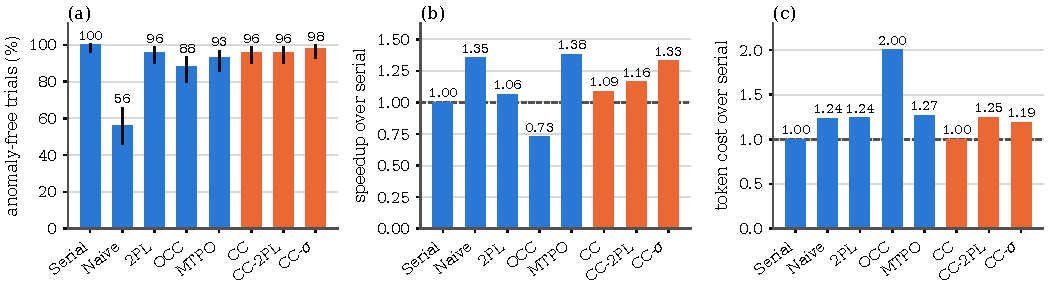
\includegraphics[width=\textwidth]{figs/main_haiku.pdf}
\caption{Claude Haiku~4.5. (a)~Anomaly-free trials over the ten scored cells,
with 95\% Wilson intervals. (b)~Mean speedup over serial execution and
(c)~mean token cost relative to serial, both over the eight contended scored
cells, on which every protocol performs the same work. Orange bars are the
certified-chopping variants.}
\label{fig:main}
\end{figure*}

Table~\ref{tab:percell} and Figure~\ref{fig:main}(a) show the Haiku results.

\paragraph{Uncoordinated agents fail, and fail structurally.}
Naive execution is anomaly-free in 56\% of trials. The three lost-update cells
fail in \emph{every} trial (0/10 each), with both models. A lost update does
not need unlucky timing: both agents must read before they write, so the
window is always open.

\paragraph{Certified chopping matches locking and exceeds repair.}
All three chopping variants are at least as safe as whole-workflow 2PL
(96\%): \cc and \cctwo at 96\% and \ccs at 98\% $[93, 99]$. \mtpo is at 93\%
$[86, 97]$. The intervals overlap, and we do not claim the differences among
the safe protocols are significant at this sample size. What the table does
show is \emph{where} each protocol loses trials. \mtpo's losses are
concentrated: 6/10 on \cell{k8s-replica-scale}, the cell where its correctness
depends on the notified agent recomputing its write. On that cell the three
chopping variants score 10/10 each, because certification merged the
read-modify-write into one piece and the interleaving \mtpo must repair never
occurs. The remaining failures of the locking-based protocols, chopping
included, are spread thinly (one or two trials on a few cells). Their final
states are not interleavings: one agent's work is missing or incomplete---an
ingress never created, one of two updates absent. Whole-workflow 2PL, which
cannot interleave at all, loses trials on the same cells in the same way. We
attribute these to the agent rather than the protocol; this model completes
its task correctly in only 78\% of trials even when run alone
(\S\ref{sec:eval:agent}).

\paragraph{A stronger model.}
With Sonnet, serial execution is correct in all 120 trials, which removes the
individual-error confound. On the ten contended cells \cc is anomaly-free in
100/100 trials, against 96/100 for 2PL, 95/100 for \mtpo and 93/100 for OCC.
\mtpo's failures are again concentrated on a repair obligation: 7/10 on
\cell{k8s-rollback-audit}, examined in \S\ref{sec:eval:agent}. \cc's only
Sonnet failures are three trials of \cell{cc-claim}, also examined there, for
an overall 117/120 (98\% $[93, 99]$).

\subsection{RQ2: Speed and cost}
\label{sec:eval:speed}

\begin{table}[t]
\caption{Aggregate results. AF: anomaly-free trials over all scored cells (10
for Haiku, 12 for Sonnet), as is cost per trial. Speedup and token cost are
relative to serial execution over the contended scored cells (8 for Haiku, 10
for Sonnet). Worst: the slowest such cell.}
\label{tab:agg}
\small
\begin{tabular}{@{}lrrrrr@{}}
\toprule
 & AF (\%) & Speedup & Worst & Tokens & \$/trial \\
\midrule
\multicolumn{6}{@{}l}{\emph{Claude Haiku~4.5}} \\
Serial   & 100 & 1.00 & 1.00 & 1.00 & 0.0124 \\
Naive    & 56  & 1.35 & 0.93 & 1.24 & 0.0150 \\
2PL      & 96  & 1.06 & 0.86 & 1.24 & 0.0147 \\
OCC      & 88  & 0.73 & 0.50 & 2.00 & 0.0240 \\
\mtpo    & 93  & \textbf{1.38} & 0.86 & 1.27 & 0.0150 \\
\cc      & 96  & 1.09 & 0.70 & \textbf{1.00} & 0.0125 \\
\cctwo   & 96  & 1.16 & 0.83 & 1.25 & 0.0146 \\
\ccs     & \textbf{98} & 1.33 & \textbf{1.08} & 1.19 & 0.0141 \\
\midrule
\multicolumn{6}{@{}l}{\emph{Claude Sonnet~5}} \\
Serial   & 100 & 1.00 & 1.00 & 1.00 & 0.0120 \\
Naive    & 75  & 1.36 & 0.95 & 1.19 & 0.0145 \\
2PL      & 97  & 1.05 & 0.81 & 1.22 & 0.0145 \\
OCC      & 94  & 0.73 & 0.52 & 1.86 & 0.0219 \\
\mtpo    & 96  & \textbf{1.43} & \textbf{1.12} & 1.20 & 0.0146 \\
\cc      & \textbf{98}  & 1.01 & 0.93 & \textbf{1.01} & 0.0125 \\
\bottomrule
\end{tabular}
\end{table}

We report speed on the contended cells, where every protocol performs the
same work. The two structural cells are discussed separately below, because on
\cell{cc-escalate} the chopping variants refuse a write that the other
protocols perform, and a protocol should not be credited for finishing sooner
by doing less. (Including both structural cells, the Haiku means are
$1.48\times$ for \ccs and $1.47\times$ for \mtpo.)

\paragraph{Contended cells.}
Figure~\ref{fig:main}(b) and Table~\ref{tab:agg} show the result. Plain \cc is
barely faster than serial ($1.09\times$ with Haiku, $1.01\times$ with Sonnet)
and no faster than 2PL. This is the expected, honest outcome. Every contended
cell has a read-modify-write or a scan-then-insert straddling the reasoning
gap, so certification merges each workflow into one piece at launch---it does
so in every trial on all ten contended cells---and the policy \emph{is}
whole-workflow locking. Certified chopping bought nothing there, and it is
important that it bought nothing rather than buying speed unsafely.

The locking discipline changes the picture. \ccs reaches $1.33\times$,
statistically indistinguishable from \mtpo's $1.38\times$
(Table~\ref{tab:boot}), and significantly faster than both 2PL and plain \cc
on every one of the eight cells. It is also the only protocol in the Haiku
run whose slowest cell is still faster than serial ($1.08\times$); 2PL and
\mtpo both bottom out at $0.86\times$ and plain \cc at $0.70\times$.

\begin{table}[t]
\caption{Paired speedup differences on the eight contended scored cells
(Haiku), with 95\% bootstrap intervals over cells and the number of cells on
which the first protocol is faster/slower.}
\label{tab:boot}
\small
\begin{tabular}{@{}lrcr@{}}
\toprule
Comparison & Mean diff. & 95\% CI & +/-- \\
\midrule
\ccs $-$ \cc     & $+0.24$ & $[+0.16, +0.33]$ & 8/0 \\
\ccs $-$ 2PL     & $+0.27$ & $[+0.17, +0.36]$ & 8/0 \\
\ccs $-$ \cctwo  & $+0.17$ & $[+0.08, +0.25]$ & 6/2 \\
\ccs $-$ \mtpo   & $-0.05$ & $[-0.29, +0.19]$ & 3/5 \\
\cctwo $-$ \cc   & $+0.08$ & $[+0.02, +0.12]$ & 5/3 \\
\cc $-$ 2PL      & $+0.03$ & $[-0.09, +0.15]$ & 3/5 \\
\bottomrule
\end{tabular}
\end{table}

\paragraph{Where chopping pays.}
On \cell{cc-claim} the certificate keeps the cut, the lock on the shared pool
is released before either agent reasons, and all work is performed (with
Haiku, every trial of every protocol completes both agents' writes). 2PL is
no faster than serial there ($0.98\times$). \cc reaches $1.73\times$, \cctwo
$1.87\times$ and \ccs $2.15\times$, against \mtpo's $1.79\times$. This is the
structure chopping exists for: the shared dependency is short and the private
interval is long.

\paragraph{Tokens.}
Figure~\ref{fig:main}(c) shows token cost. Plain \cc costs the same as serial
execution ($1.00\times$): it never aborts and never notifies, so no inference
is repeated and no context is added. \ccs costs $1.19\times$, below 2PL
($1.24\times$) and \mtpo ($1.27\times$). The two faster protocols pay in
different currencies, which Table~\ref{tab:mech} separates: \ccs runs more
rounds than \mtpo (8.2 against 7.7 per trial) because wounded agents redo
work, but \mtpo spends more tokens in total (7{,}339 against 6{,}810)
because every notification adds its payload, and the reasoning about it, to
the agent's context.

\subsection{RQ3: Locking disciplines}
\label{sec:eval:locking}

\begin{table}[t]
\caption{Mechanism counts per trial over the ten scored cells (Haiku),
recovered from runtime traces.}
\label{tab:mech}
\small
\begin{tabular}{@{}lrrrrrr@{}}
\toprule
 & Deadl. & Wounds & Aborts & Notif. & Rounds & Tokens \\
\midrule
Serial & 0 & 0 & 0 & 0 & 6.9 & 6{,}104 \\
2PL    & 0.76 & 0 & 0.76 & 0 & 8.5 & 7{,}077 \\
\mtpo  & 0 & 0 & 0 & 0.80 & 7.7 & 7{,}339 \\
\cc    & 0 & 0 & 0 & 0.10 & 7.1 & 6{,}245 \\
\cctwo & 0.80 & 0 & 0.80 & 0.10 & 8.6 & 7{,}076 \\
\ccs   & 0 & 0.78 & 0.78 & 0.10 & 8.2 & 6{,}810 \\
\bottomrule
\end{tabular}
\end{table}

\begin{figure}[t]
\centering
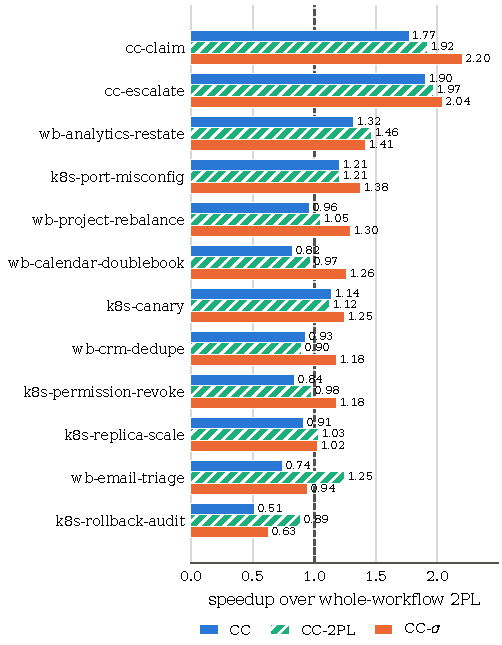
\includegraphics[width=\columnwidth]{figs/percell_haiku.pdf}
\caption{Speedup of each locking discipline over whole-workflow 2PL, per cell
(Haiku, all twelve cells). On the dashed line a protocol is no better than
2PL. \ccs trails 2PL only on the two cells at the bottom, which are the two
contended cells on which 2PL never deadlocks.}
\label{fig:percell}
\end{figure}

Table~\ref{tab:mech} and Figure~\ref{fig:percell} compare the three
disciplines.

\paragraph{Deadlock is the common case for incremental locking.}
\cctwo deadlocks 0.80 times per trial, slightly more often than
whole-workflow 2PL (0.76). The cause is the lock-upgrade pattern: both agents
read an object and both then try to write it. \cc never deadlocks, by
construction, and \ccs never deadlocks, by Proposition~\ref{prop:acyclic}; we
observed zero deadlocks in 120 trials of each.

\paragraph{Prevention beats detection.}
\ccs aborts as often as \cctwo (0.78 wounds against 0.80 deadlock aborts per
trial) and yet is significantly faster ($+0.17\times$,
Table~\ref{tab:boot}). The difference is \emph{when} the abort happens. A
wound is issued at the moment of conflict. A deadlock is resolved only after
both agents have blocked and the cycle has been found, and each has by then
spent a model inference producing the call on which it blocked.

We had expected aborts to be expensive to undo. They were not: all 76 deadlock
aborts of 2PL and all 80 of \cctwo, and 86 of the 90 wounds of \ccs, undid
zero writes. In these workloads the victim has read but not yet written, so
the cost of an abort is the repeated inference, not the compensation.

\paragraph{No starvation observed.}
The restart cap was never reached. Of the 100 scored \ccs trials, 78 contained
a wound, and all 78 ended anomaly-free; the two \ccs failures occurred in
trials with no wound.

\paragraph{Where \ccs loses: wounding without a deadlock to prevent.}
Figure~\ref{fig:percell} shows \ccs ahead of plain \cc on all twelve cells and
ahead of 2PL on ten. The two exceptions, \cell{wb-email-triage}
($0.94\times$) and \cell{k8s-rollback-audit} ($0.63\times$), follow an exact
rule. Across the twelve cells, 2PL deadlocks at a mean rate of 0.76 per trial
on the ten cells where \ccs beats it, and \emph{never} on the two where \ccs
loses. On those two cells contention is mild: 2PL resolves it by a short wait
and no abort. Wound-wait cannot tell a conflict that would have resolved
itself from one that would have deadlocked. It aborts the lower-priority
holder either way and so converts a short wait into a redo. \cctwo, which
aborts only on an actual cycle, is the fastest of the three disciplines on
exactly these two cells ($1.25\times$ and $0.89\times$). The two cells are the ones excluded
from Haiku aggregates, so this cost does not appear in Table~\ref{tab:agg}; we
report it here because it identifies the next refinement, discussed in
\S\ref{sec:discussion}.

\subsection{RQ4: Dependence on the agent}
\label{sec:eval:agent}

\begin{table}[t]
\caption{The two agent assumptions behind repair-based concurrency control,
measured. A1: serial trials whose final state exactly matches a reference.
A3: \mtpo trials with a notification that end anomaly-free.}
\label{tab:assump}
\small
\begin{tabular}{@{}lrr@{}}
\toprule
 & A1 (individual success) & A3 (self-healing) \\
\midrule
Assumed in~\cite{lyu2026coagent} & 98\% & 95\% \\
Claude Haiku~4.5 & 78\% & 71/78 = 91\% $[83, 96]$ \\
Claude Sonnet~5  & 100\% & 95/100 = 95\% $[89, 98]$ \\
\bottomrule
\end{tabular}
\end{table}

Every protocol depends on the agent for something. The question is for what,
and what happens when the agent falls short.

\paragraph{A1 moves with the model; A3 barely does.}
Table~\ref{tab:assump} measures the two assumptions. Individual success rises
from 78\% to 100\% between the two models. Self-healing rises only from 91\%
to 95\%. The stronger model fixes nearly all of its individual errors but
remains about one time in twenty unable to discharge a repair obligation. To
the extent two models can show it, repair looks like a structural residual
rather than a capability gap that the next model closes.

\paragraph{How repair fails.}
\cell{k8s-rollback-audit} makes the residual concrete. Agent $A$ rolls a
deployment back and logs that it did; agent $B$ appends an audit record naming
the image it observed. Under \mtpo with Sonnet, $A$'s record lands first, $B$
is notified that the image changed, and $B$ must retract its record and file a
corrected one. In seven of ten trials it does. In two it appends a
\emph{second} record instead of replacing the first; an append has no
inverse, so the log is left with a duplicate that no serial order produces. In
one it ignores the notification and files the stale value. \cc scores 10/10 on
this cell with Sonnet: the read and the append are in one sealed piece, and no
notification is ever sent.

\paragraph{Certified chopping relocates the obligation.}
It would be wrong to conclude that certified chopping is independent of the
agent. Its obligation is elsewhere: an agent whose call is \emph{refused}
must carry on correctly. \cell{cc-claim} with Sonnet shows both the
obligation and a subtlety of model-driven plans. Agent $B$'s task is a blind
write to the shared pool followed by a private write, and its certified plan
has one piece for each. Sonnet, more cautious than the task requires, first
\emph{reads} the pool. That read is permitted by the footprint of the piece
that was certified for the write, so it runs, and the piece closes when the
call returns. The write that follows now needs a new piece. Together with the
committed one it would close a mixed cycle through the other agent's read of
the pool, so the revision is refused, correctly by
Corollary~\ref{cor:imp}. The model's improvisation spent the piece its plan
had been certified with.

What happens next is up to the agent. Sonnet read first in nine trials of
ten. In the tenth it wrote blind, as instructed, and both writes completed. In
six it proceeded to its private write, leaving the pool update undone. In three it treated the
refusal as terminal and stopped, leaving its private claim unwritten as well;
these are \cc's three Sonnet failures. With Haiku, which performs the blind
write as instructed, the same cell completes fully in every trial.

\paragraph{Fail-safe against fail-dirty.}
The two failure modes are not symmetric. When \mtpo's obligation is not met,
shared state is corrupted in a way the system cannot undo: a duplicate or
stale record in an append-only log. When certified chopping's obligation is
not met, shared state is clean and serializable but an intent is unfinished,
and a retry would still complete it. A refusal is also visible to the runtime,
which knows exactly which call it refused, whereas an unperformed repair
looks, from outside, like an agent that decided no repair was needed.

\paragraph{Redo is easier than repair.}
\ccs asks a third thing of the agent: after a wound, do the task again from
the beginning. With Haiku, all 78 wounded trials on the scored cells ended
anomaly-free, a 100\% success rate $[95, 100]$, where the same model
discharges \mtpo's repair obligation in 91\% of notified trials. The
difference is plausibly the kind of reasoning required. A wounded agent
receives its original task and a fresh context; it is not asked to work out
which of its past operations a change invalidates.

\subsection{Mid-flight revisions}
\label{sec:eval:revisions}

\begin{table}[t]
\caption{Outcomes of mid-flight revisions. Top: durable runtime, 220 revisions
per contention level over 10 seeds. Bottom: live agents under \cc.}
\label{tab:admit}
\small
\begin{tabular}{@{}lrrrrr@{}}
\toprule
 & Revisions & Admitted & Coarsened & Refused & Rate \\
\midrule
1 shared pool  & 220 & 10 & 0 & 210 & 4\% \\
2 shared pools & 220 & 20 & 0 & 200 & 9\% \\
4 shared pools & 220 & 37 & 0 & 183 & 17\% \\
8 shared pools & 220 & 73 & 9 & 138 & 37\% \\
\midrule
Haiku agents   & 10 & 0 & 0 & 10 & 0\% \\
Sonnet agents  & 32 & 6 & 0 & 26 & 19\% \\
\bottomrule
\end{tabular}
\end{table}

Table~\ref{tab:admit} reports what admission decided. In the durable runtime,
where workflows escalate into one of $k$ shared pools after committing a
prefix, between 4\% and 37\% of revisions are admissible, rising as contention
is spread over more pools. The rest are refused because the residual cycle
passes through a committed piece. No admitted revision produced a
non-serializable history or violated an invariant.

With live agents, revisions arise only on the two structural cells. Haiku
produces ten, all on \cell{cc-escalate}, the executable witness of
Figure~\ref{fig:witness}; all ten are refused, the shared item is untouched in
every trial, and the final state is serializable. That 0\% is a correctness
result on a cell built to be inadmissible, not an estimate of an admission
rate. Sonnet's additional reads generate more revisions, 32 across both
cells, of which six are admitted.

This is the most important limitation we measured. Prefix-aware
recertification decides the question correctly and cheaply and never admits an
unsafe revision, but the answer is frequently no.

\subsection{Mechanism study on a durable store}
\label{sec:eval:mechanism}

The agent study has two agents per cell and an in-memory store. The mechanism
study complements it with the durable runtime: 32 workflows per batch on 8
worker threads against SQLite, 4 shared pools, 10 seeds per configuration,
and real wall-clock time. Reasoning is a 50\,ms calibrated delay rather than
model inference, so these are mechanism measurements, not agent latencies.
The baselines are a whole-workflow database transaction, whole-workflow 2PL
over the union footprint, whole-workflow OCC with read validation and range
re-scan, and \emph{unchecked chopping}, which executes the fine pieces with no
certification and serves as an unsafe control. Correctness is judged by
recording every mediated operation and testing the workflow-level
serialization graph of the actual history for cycles.

\begin{table}[t]
\caption{Durable runtime: speedup over a whole-workflow database transaction
(makespan, 10 seeds). Last column: seeds in which unchecked chopping produced
a non-serializable history and violated the application invariant.}
\label{tab:durable}
\small
\begin{tabular}{@{}lrrrrr@{}}
\toprule
Workload & 2PL & OCC & \cc & Unchecked & Unsafe \\
\midrule
claim    & 3.19 & 2.99 & \textbf{7.35} & 7.24 & 0/10 \\
budget   & 3.06 & 2.90 & 3.10 & 7.18 & 10/10 \\
retail   & 3.11 & 2.93 & 3.07 & 7.41 & 10/10 \\
calendar & 3.13 & 2.92 & 3.07 & 7.34 & 10/10 \\
replan   & 5.11 & \textbf{7.61} & 7.14 & 7.58 & 0/10 \\
escalate & 3.04 & 4.51 & \textbf{6.24} & 5.91 & 10/10 \\
\bottomrule
\end{tabular}
\end{table}

\paragraph{Throughput.}
Table~\ref{tab:durable} shows the same two regimes as the agent study, at
sixteen times the concurrency. On \emph{claim}, certification keeps all 96
pieces: \cc is $7.35\times$ faster than a whole-workflow transaction and
$2.4\times$ faster than whole-workflow 2PL, and 95th-percentile latency falls
from 1.96\,s to 0.12\,s. On \emph{budget}, \emph{retail} and \emph{calendar},
which have a read-modify-write or scan-then-insert across the reasoning gap,
certification merges the pieces and \cc performs as whole-workflow locking
does, within seed-to-seed noise. Unchecked chopping is about $2.4\times$
faster still on those three workloads and is non-serializable, with a violated
invariant, in all ten seeds of each; on \emph{calendar} it double-books rooms
although each workflow's logic is individually correct. On \emph{escalate},
where two thirds of workflows revise their plan mid-flight, prefix-aware
admission gives $6.24\times$ against $3.04\times$ for 2PL, with no
violations. No safe policy produced a non-serializable history in any seed.

\paragraph{Sensitivity.}
The benefit tracks contention structure and available concurrency, not
reasoning time alone. On \emph{claim}, the speedup of \cc over
whole-workflow 2PL is $5.99\times$ with one shared pool and $1.30\times$ with
sixteen, where there is little contention to relieve; $0.99\times$ with one
worker thread and $3.12\times$ with sixteen. With zero reasoning time it is
$0.59\times$: chopping is a net loss when there is no private interval to
release a lock for, because each extra piece boundary costs a commit. On
\emph{budget} the ratio stays between $0.82\times$ and $1.06\times$
throughout, as it must, since certification always merges that workload back
to whole-workflow locking.

\paragraph{Certification cost.}
Static certification takes 28.5\,ms for 32 workflows (96 pieces) and 131\,ms
for 128 workflows (384 pieces); indexing conflict candidates and repairing
every mixed block per pass brought the latter down from 22\,s for a naive
all-pairs implementation. Readmission is cheaper, 0.6\,ms and 5.0\,ms at the
same sizes, because the frontier constrains the search. The cost is not
always worth paying: certifying \emph{budget} costs 35\,ms against a batch
that runs for 0.68\,s and purchases no speedup. A deployment should cache
certificates per program template and recertify only on structural change.

\paragraph{Crash and recovery.}
Three workflows each move 10 units between a private pair of accounts, in two
pieces. There are no cross-workflow conflicts, so certification accepts the
chopping: the batch is isolation-safe and still not failure-atomic. Killing
the process after a debit piece commits leaves one pair broken and the batch
total at 5{,}990 instead of 6{,}000. Without durable continuation the damage
is permanent. With it, recovery resumes the workflow from its progress record
and restores the total. A crash \emph{inside} a piece's transaction rolls back
the writes together with the progress record, confirming that pieces are
atomic.
